% !TeX root = ./main.tex
% !TEX program = xelatex

\documentclass[12pt]{article}
\usepackage[table]{xcolor}
\usepackage{graphicx}
\usepackage{longtable}

\usepackage{fullpage}
\usepackage{enumitem}
\usepackage{booktabs}
\usepackage{makecell}
\usepackage{amsmath}
\usepackage{tikz}
\usetikzlibrary{arrows}
\usepackage{listings}
\usepackage{algorithm}
\usepackage[noend]{algpseudocode}
\usepackage{multicol}
\usepackage{microtype}
\usepackage{graphicx}
\usepackage[export]{adjustbox}
\usepackage{hyperref}
\hypersetup{
    colorlinks,
    citecolor=black,
    filecolor=black,
    linkcolor=black,
    urlcolor=black
}
\newcommand{\myparagraph}[1]{\paragraph{#1}\mbox{}\\}


%% Language and font encodings
\usepackage[utf8]{inputenc}
\usepackage{xunicode}
\usepackage{xltxtra}
\usepackage{amsfonts, amsmath}
\usepackage[english,greek]{babel}
\usepackage{tcolorbox}

%\usepackage{xgreek}

\setmainfont[Mapping=tex-text]{CMU Serif}
\begin{document}
\sloppy
\begin{titlepage}



\newcommand{\HRule}{\rule{\linewidth}{0.5mm}}
\center

\includegraphics[width=50mm,scale=0.5]{imgs/logo.png}\\[1cm]
\textsc{\LARGE ΕΘΝΙΚΟ ΜΕΤΣΟΒΙΟ ΠΟΛΥΤΕΧΝΕΙΟ}\\[0.05cm] % Name of your university/college
\textsc{\textbf{\Large ΣΧΟΛΗ ΗΛΕΚΤΡΟΛΟΓΩΝ ΜΗΧΑΝΙΚΩΝ \\ \& ΜΗΧΑΝΙΚΩΝ ΥΠΟΛΟΓΙΣΤΩΝ}}\\[1.cm] % Major heading such as course name

\vspace{05mm}
\HRule \\[0.4cm]
{ \huge \bfseries Άσκηση 4 - Προηγμένα Θέματα Αρχιτεκτονικής Υπολογιστών }\\[0.4cm] 
\HRule \\[1.5cm]
 
\center
{\Large Γρηγόριος Θανάσουλας \\ \vspace{1em} gregthanasoulas@gmail.com \\ \vspace{5mm} \Large A.M: 03114131} \\
\vspace{15mm}

{\large \today} % Date, change the \today to a set date if you want to be precise
\vfill

\end{titlepage}
\newpage
\tableofcontents
\newpage

\large{
\setcounter{tocdepth}{3}
\setcounter{secnumdepth}{3}
\section{Σκοπός}
\vspace{3mm}

Η άσκηση αυτή αποσκοπεί στη μελέτη των μηχανισμών συγχρονισμού και των
πρωτοκόλλων συνάφειας κρυφής μνήμης (cache coherence protocols) σε σύγχρονες
πολυπύρηνες αρχιτεκτονικές. Για την αξιολόγηση των μηχανισμών, χρησιμοποιείται
το εργαλείο Sniper ώστε να προσομοιωθεί ένα πολυπύρηνο σύστημα με διαφορετικούς
μηχανικούς συγχρονισμού.


\vspace{3mm}

\section{Πειραματική Αξιολόγηση}
\subsection{Ερώτημα 3-1-1}

\begin{minipage}{\textwidth}
   \begin{center}
      \fbox{\textlatin{\textbf{\textit{Grain Size: 1}}}}\\
      \vspace{3mm}
      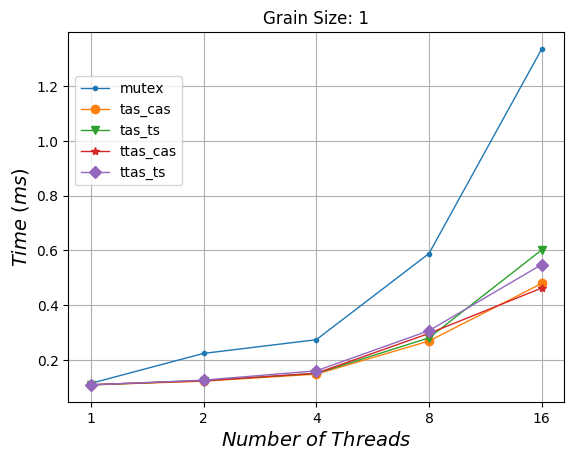
\includegraphics[width=0.7\textwidth, frame]{./graphs/time/grain-1.png}
      \vspace{6mm}
   \end{center}
\end{minipage}

\begin{minipage}{\textwidth}
   \begin{center}
      \fbox{\textlatin{\textbf{\textit{Grain Size: 10}}}}\\
      \vspace{3mm}
      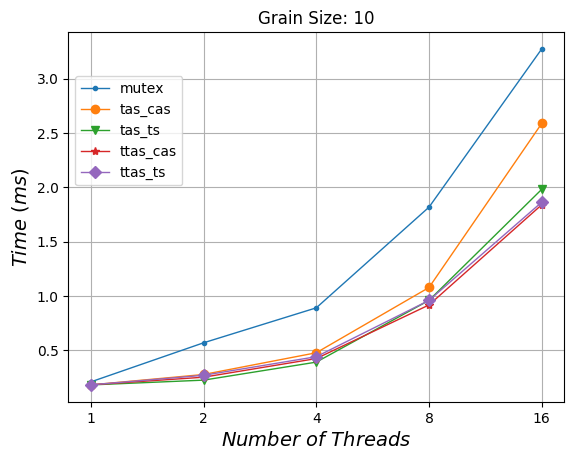
\includegraphics[width=0.7\textwidth, frame]{./graphs/time/grain-10.png}
      \vspace{6mm}
   \end{center}
\end{minipage}

\begin{minipage}{\textwidth}
   \begin{center}
      \fbox{\textlatin{\textbf{\textit{Grain Size: 100}}}}\\
      \vspace{3mm}
      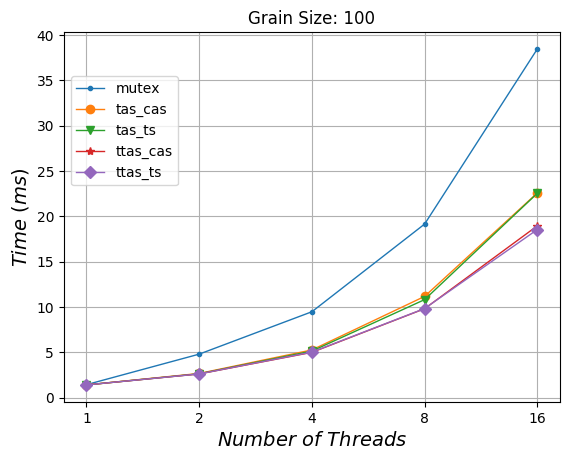
\includegraphics[width=0.7\textwidth, frame]{./graphs/time/grain-100.png}
      \vspace{6mm}
   \end{center}
\end{minipage}

\subsection{Ερώτημα 3-1-2}
\vspace{1em}
\subsection{Ερώτημα 3-1-3}
Ακολουθούν τα διαγράμματα της ενέργειας αλλά και της μετρικής EDP (Energy Delay Product)
για τα προηγούμενα πειράματα: 
\begin{minipage}{\textwidth}
   \begin{center}
      \fbox{\textlatin{\textbf{\textit{Grain Size: 1}}}}\\
      \vspace{3mm}
      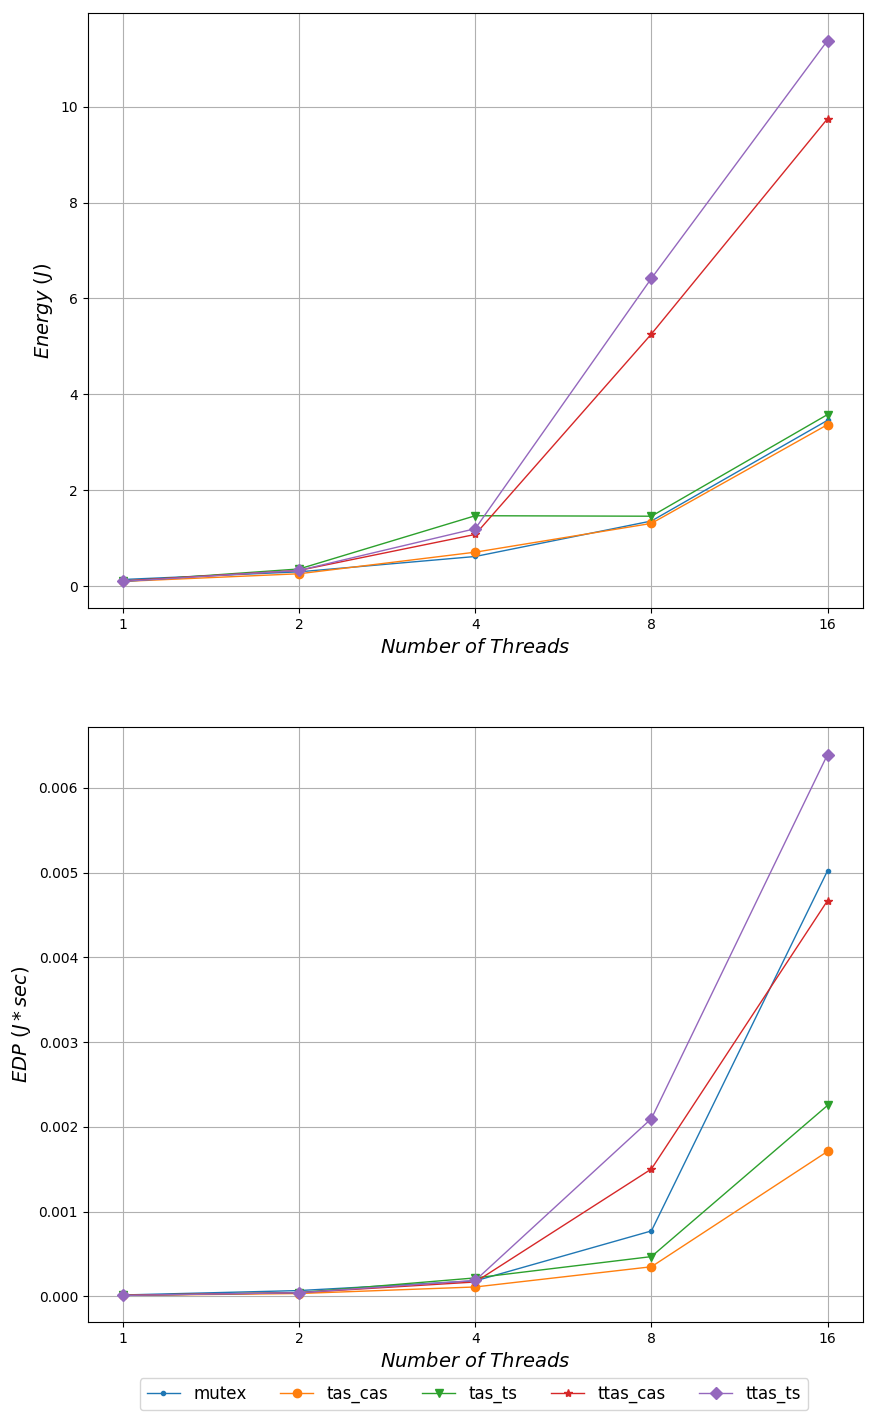
\includegraphics[width=0.7\textwidth]{./graphs/sniper/energy/grain-1.png}
      \vspace{6mm}
   \end{center}
\end{minipage}

\begin{minipage}{\textwidth}
   \begin{center}
      \fbox{\textlatin{\textbf{\textit{Grain Size: 10}}}}\\
      \vspace{3mm}
      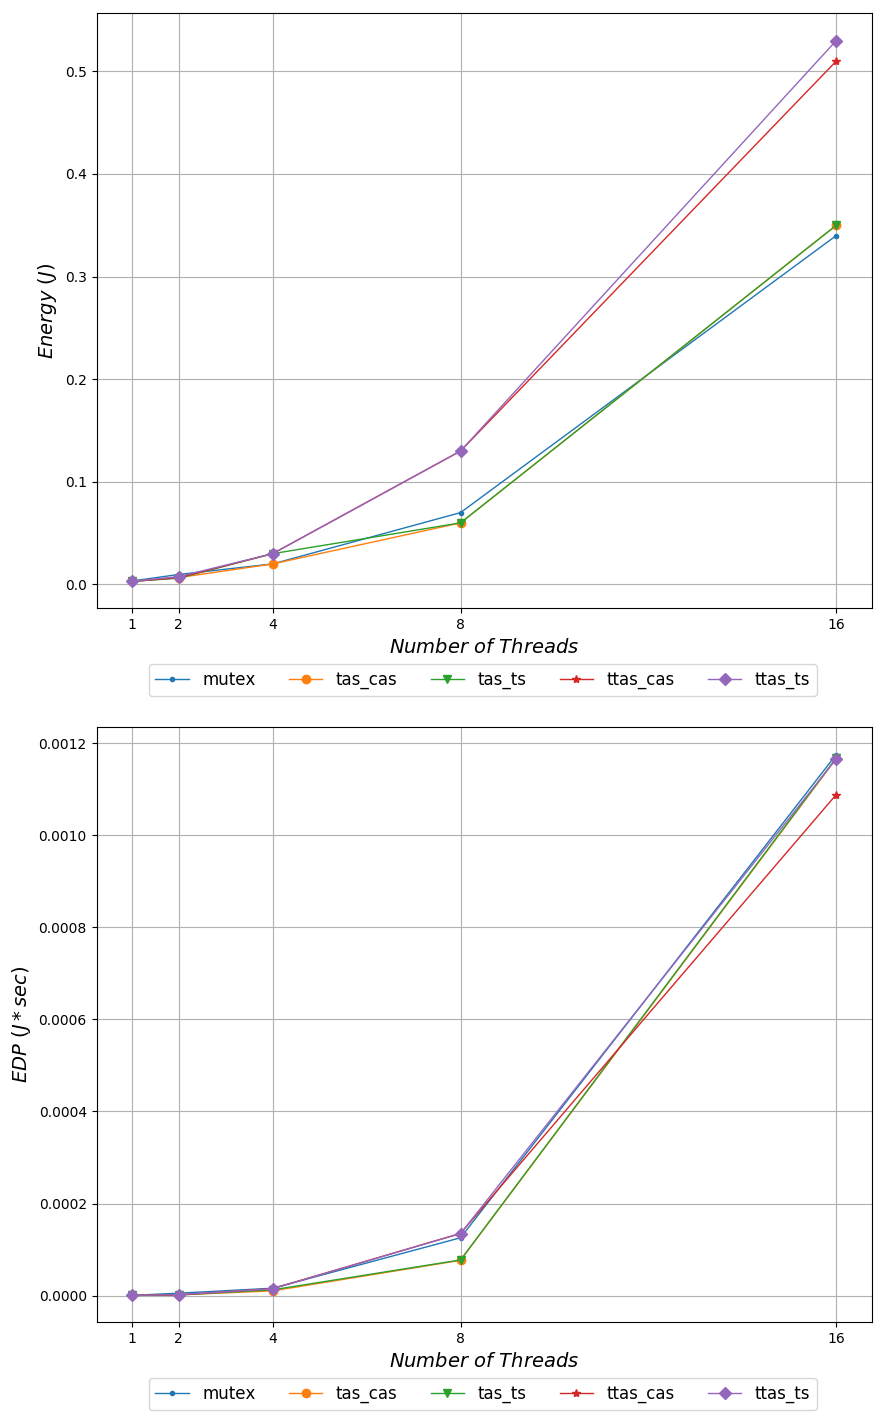
\includegraphics[width=0.7\textwidth]{./graphs/sniper/energy/grain-10.png}
      \vspace{6mm}
   \end{center}
\end{minipage}

\begin{minipage}{\textwidth}
   \begin{center}
      \fbox{\textlatin{\textbf{\textit{Grain Size: 100}}}}\\
      \vspace{3mm}
      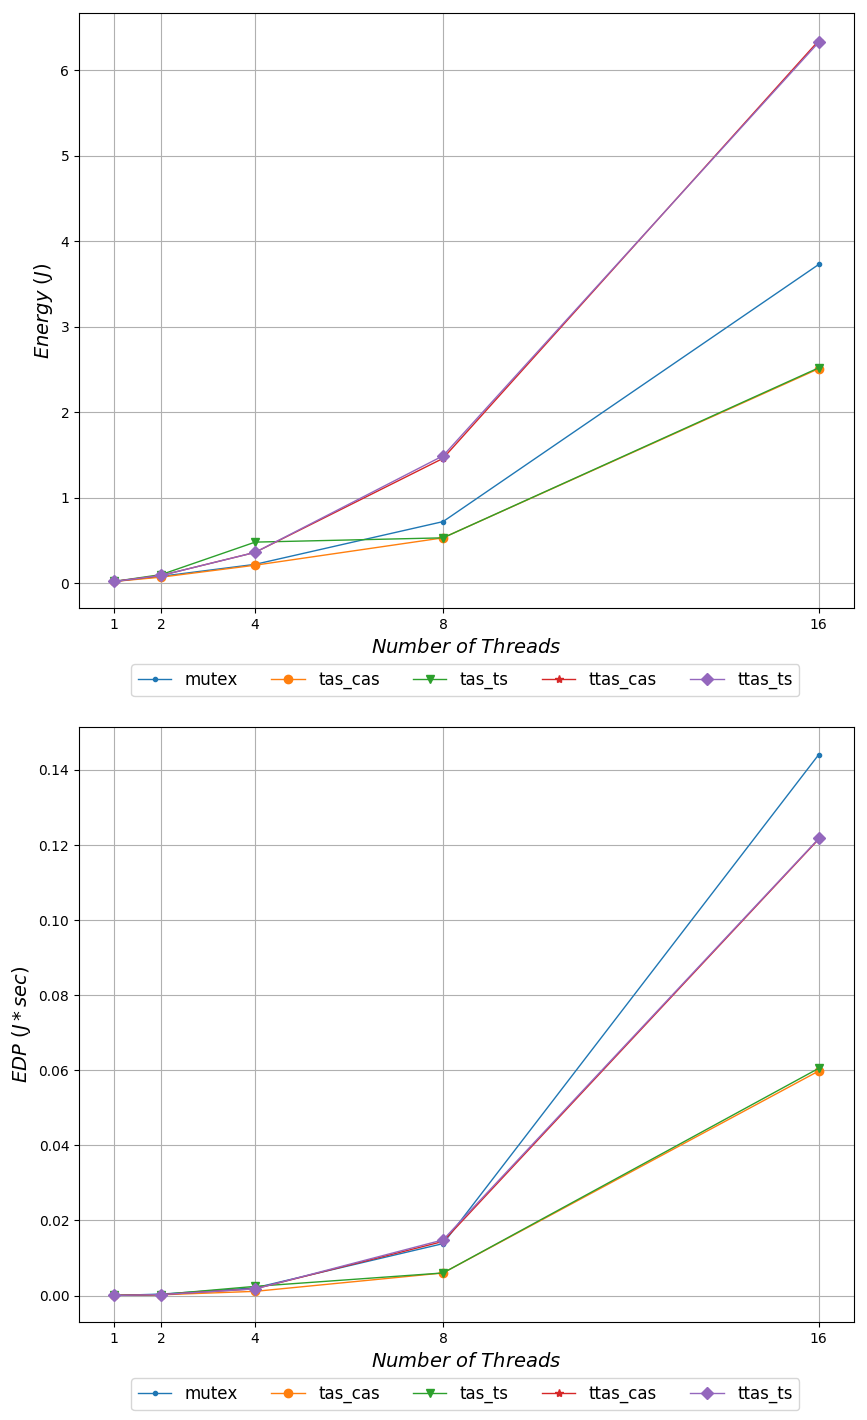
\includegraphics[width=0.7\textwidth]{./graphs/sniper/energy/grain-100.png}
      \vspace{6mm}
   \end{center}
\end{minipage}

\paragraph{Σχόλια - Συμπεράσματα:}
Παρατηρούμε πως η ενέργεια αυξάνεται σχεδόν εκθετικά με το πλήθος των νημάτων.
Ειδικότερα όταν το πλήθος αυτό γίνει από 8 νήματα σε 16 η ενέργεια που καταναλώνεται
είναι σημαντικά μεγάλη. 

Επίσης, βλέπουμε πως για μεγαλύτερα grain size 10 και 100, οι μηχανισμοί
TTAS\_CAS και TTAS\_TS σημειώνουν πολύ υψηλότερη κατανάλωση ενέργειας για μεγάλο
αριθμό νημάτων σε σχέση με τις υπόλοιπες υλοποιήσεις. Αυτό αιτιολογείται από το
γεγονός ότι κάθε νήμα που προσπαθεί να πάρει το κατειλημμένο lock κάνει τοπικά
sniping πάνω στην cache του με συνεχόμενα reads τα οποία κοστίζουν ενεργειακά
πολύ περισσότερο συγκριτικά με τα τα stalls εξαιτίας cache miss ή κατειλημμένο
bus που εμφανίζονται στην περίπτωση των Test-and-set υλοποιήσεων. Σε όλες τις
παραπάνω περιπτώσεις φθηνότερο ενεργειακά φαίνεται να είναι ο μηχανισμός TAS.

Αναφορικά με τη μετρική EDP, αξίζει να σημειώσουμε ότι για grain size 10 οι
καμπύλες τείνουν να ταυτιστούν, και άρα οι μηχανισμοί μπορούν να θεωρηθούν
εξίσου καλοί από πλευρά Energy Delay Product. Στη γενική περίπτωση όμως, με αυτό
το κριτήριο κερδίζουν οι μηχανισμοί TAS-CAS και TAS-TS. Όσον αφορά το μηχανισμό
MUTEX έχει τη χειρότερη επίδοση κρίνοντας με τη μετρική EDP για μεγάλο πλήθος
νημάτων (>8), ανεξαρτήτως grain size.
\subsection{Ερώτημα 3-1-4}

\begin{minipage}{\textwidth}
   \begin{center}
      \fbox{\textlatin{\textbf{\textit{Time analysis}}}}\\
      \vspace{3mm}
      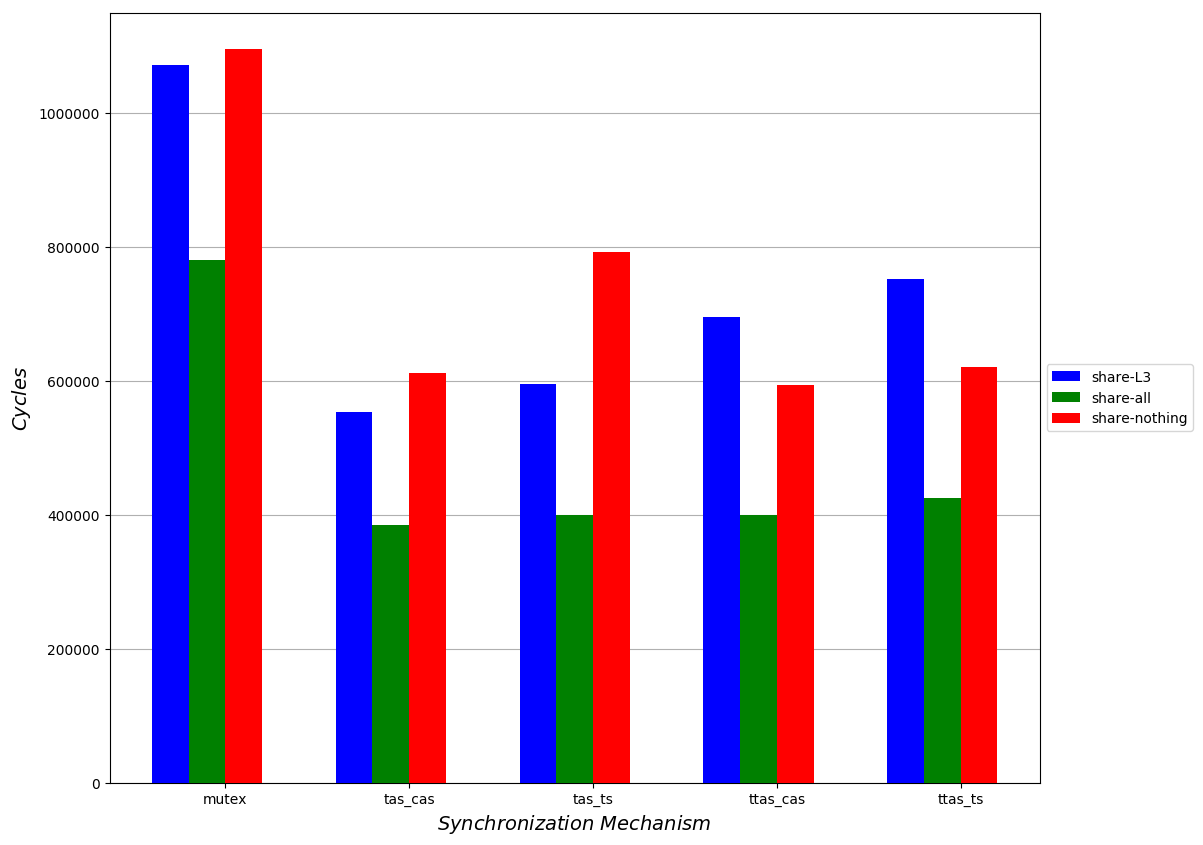
\includegraphics[width=0.75\textwidth, frame]{./graphs/sniper/threads/topology-time-analysis.png}
      \vspace{6mm}
   \end{center}
\end{minipage}
\\
\begin{minipage}{\textwidth}
   \begin{center}
      \fbox{\textlatin{\textbf{\textit{Energy Analysis}}}}\\
      \vspace{3mm}
      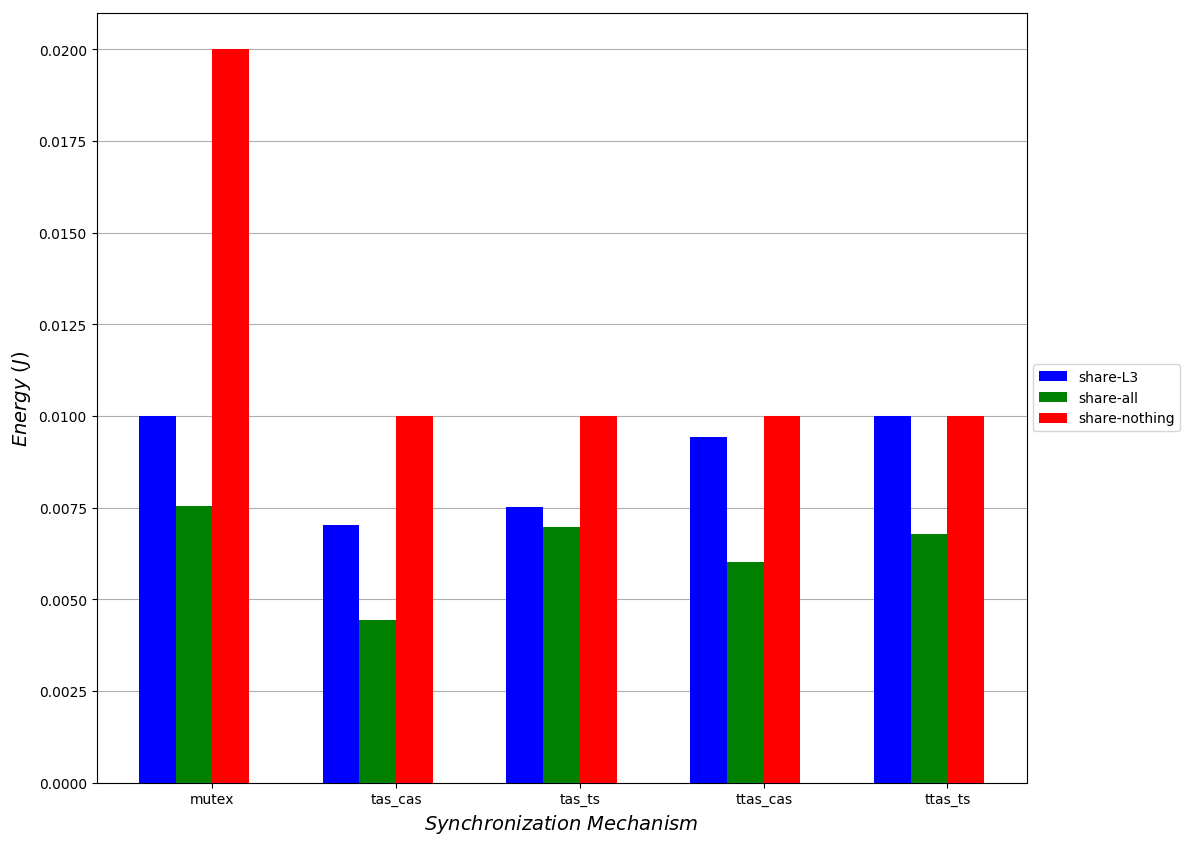
\includegraphics[width=0.75\textwidth, frame]{./graphs/sniper/threads/topology-energy-analysis.png}
      \vspace{6mm}
   \end{center}
\end{minipage}

\begin{minipage}{\textwidth}
   \begin{center}
      \fbox{\textlatin{\textbf{\textit{EDP Analysis}}}}\\
      \vspace{3mm}
      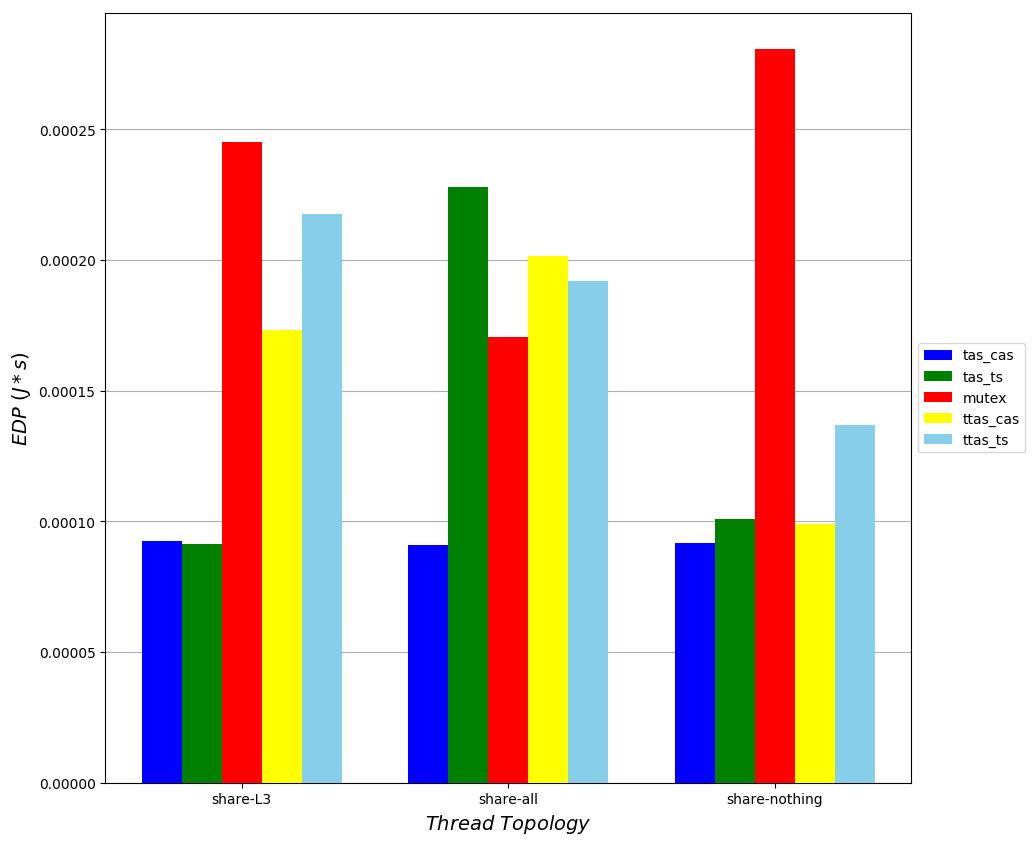
\includegraphics[width=0.75\textwidth, frame]{./graphs/sniper/threads/topology-edp-analysis.png}
      \vspace{6mm}
   \end{center}
\end{minipage}
\subsection{Ερώτημα 3-2}

Σε αυτό το τμήμα της άσκησης εξετάζουμε την επίδοση των κάτωθι διαφορετικών
τοπολογιών που διαφέρουν μεταξύ τους ως προς τον διαμοιρασμό των κρυφών μνημών.
Συγκεκριμένα εξετάζουμε τις ακόλουθες τοπολογίες:

\begin{itemize}
   \item share-all: και τα 4 νήματα βρίσκονται σε πυρήνες με κοινή L2 cache
   \item share-L3: και τα 4 νήματα βρίσκονται σε πυρήνες με κοινή L3 cache, αλλά όχι κοινή L2
   \item share-nothing: και τα 4 νήματα βρίσκονται σε πυρήνες με διαφορετική L3 cache 
\end{itemize}

\begin{minipage}{\textwidth}
   \begin{center}
      \vspace{10mm}
      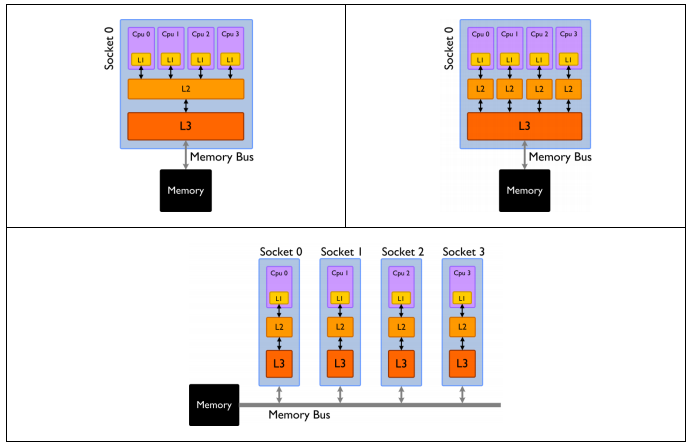
\includegraphics[width=0.9\textwidth]{./imgs/topologies.png}
      \vspace{6mm}
   \end{center}
\end{minipage}

\noindent Στη συνέχεια ακολουθούν ραβδογράμματα τα οποία παρουσιάζουν τους χρόνους
εκτέλεσης, την κατανάλωση ενέργειας και την μετρική EDP για τα configurations
αυτά:

\begin{minipage}{\textwidth}
   \begin{center}
      \fbox{\textlatin{\textbf{\textit{Time analysis}}}}\\
      \vspace{3mm}
      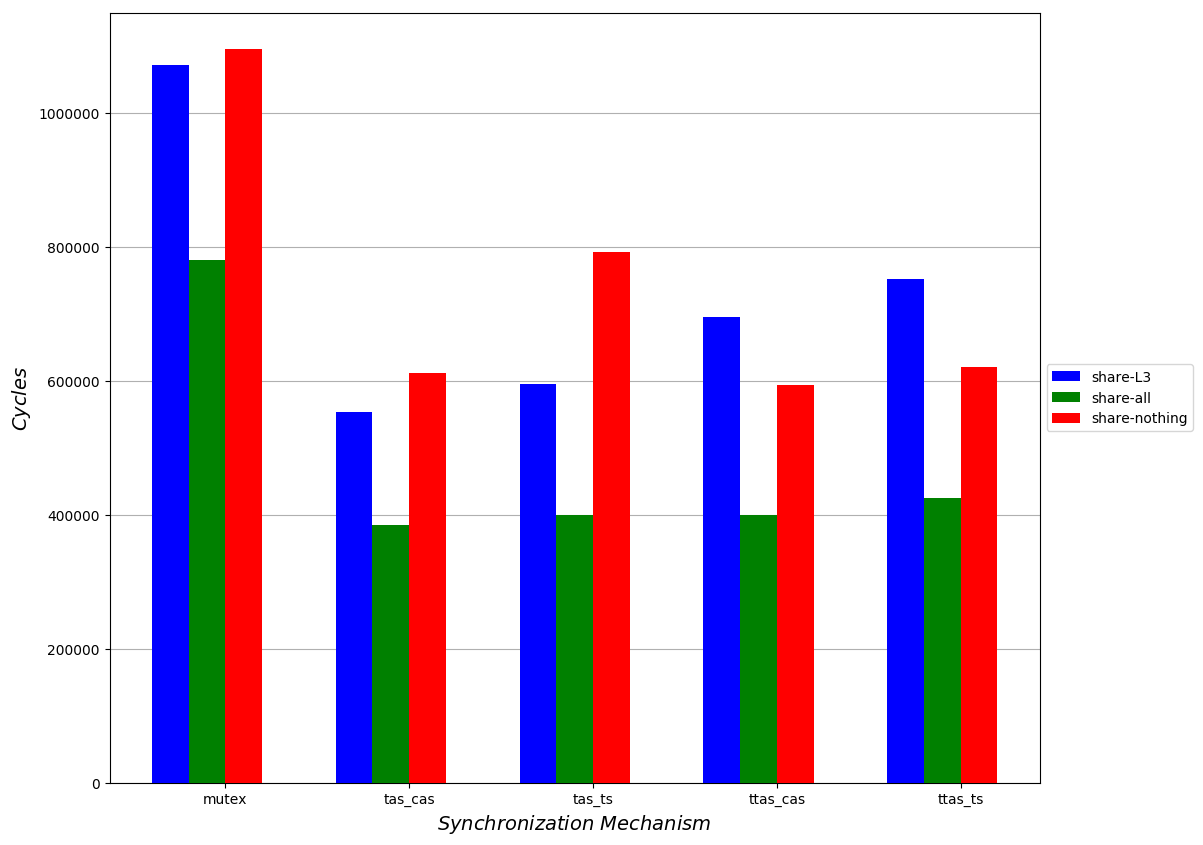
\includegraphics[width=0.75\textwidth, frame]{./graphs/sniper/threads/topology-time-analysis.png}
      \vspace{6mm}
   \end{center}
\end{minipage}

\begin{minipage}{\textwidth}
   \begin{center}
      \fbox{\textlatin{\textbf{\textit{Energy Analysis}}}}\\
      \vspace{3mm}
      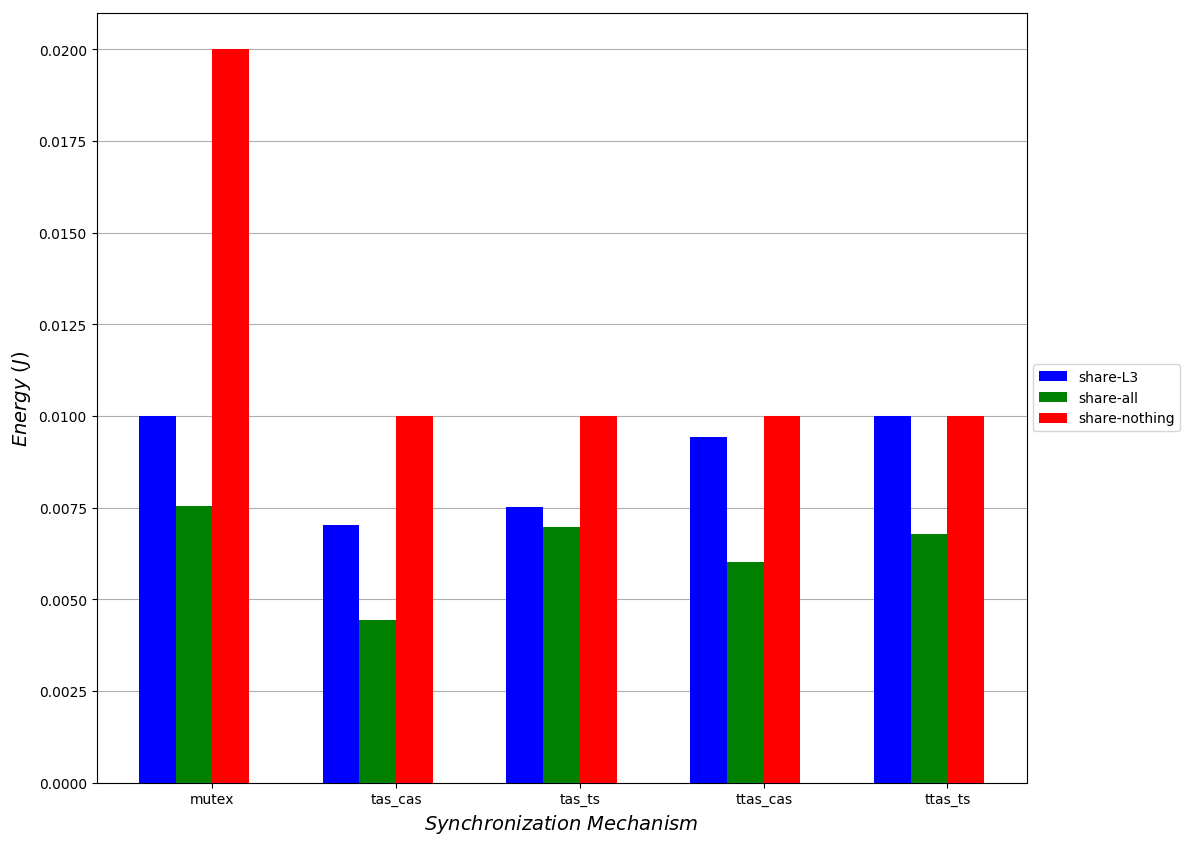
\includegraphics[width=0.75\textwidth, frame]{./graphs/sniper/threads/topology-energy-analysis.png}
      \vspace{6mm}
   \end{center}
\end{minipage}

\begin{minipage}{\textwidth}
   \begin{center}
      \fbox{\textlatin{\textbf{\textit{EDP Analysis}}}}\\
      \vspace{3mm}
      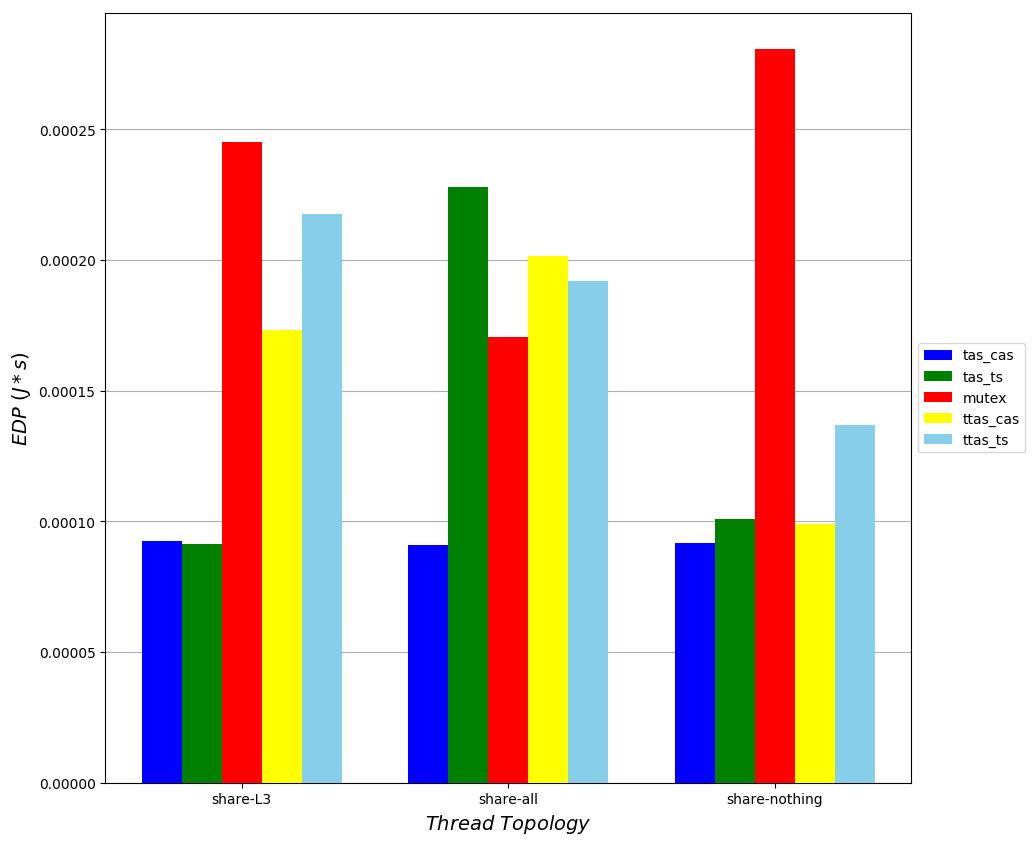
\includegraphics[width=0.75\textwidth, frame]{./graphs/sniper/threads/topology-edp-analysis.png}
      \vspace{6mm}
   \end{center}
\end{minipage}

\paragraph{Συμπεράσματα - Σχόλια}
Όσον αφορά την επίδοση με βάση τη μετρική του χρόνου (ή αντίστοιχα κύκλος
εκτέλεσης) για όλους τους υπο μελέτη μηχανισμούς συγχρονισμου, την καλύτερη
επίδοση λαμβάνουμε στην τοπολογία \textbf{share-all}. Για τους μηχανισμούς
συγχρονισμού MUTEX, TAS\_TS, TAS\_CAS οι τοπολογίες σε φθίνουσα επίδοση είναι οι
share-all, share-L3, share-nothing. Για τους μηχανισμούς συγχρονισμού TTAS\_TS,
TTAS\_CAS οι τοπολογίες σε φθίνουσα επίδοση είναι οι share-all, share-nothing,
share-L3. Η βέλτιστη επίδοση του share-all αιτιολογείται από το γεγονός οτι αν
επεξεργαστής ζητήσει ένα Invalid cache line θα ενημερωθεί η ιεραρχία μνήμης
μέχρι την L2 και θα το διαβάσει από εκεί, ενώ στο share-L3 η invalid cache line
θα ζητηθεί από την L3 και για share-nothing φτάνουμε μέχρι και την κύρια μνήμη
για κάθε αυξάνοντας σημαντικά τον χρόνο που απαιτείται, αφού όσο πιο "μακριά"
ιεραρχικά βρίσκεται μία μνήμη από τον επεξεργαστή τόσο πιο αργή είναι.

Ως προς την κατανάλωση ενέργειας την μεγαλύτερη κατανάλωση έχουμε στην τοπολογία 
share-nothing, ενώ την μικρότερη κατανάλωση στην τοπολογία share-all. Αντίστοιχα,
με κριτήριο την EDP μετρική, την καλύτερη επίδοση έχει η τπολογία share-all.
\vspace{1em}

\noindent Ακολουθεί η υλοποίηση των μηχανισμών στο αρχείο lock.h: \vspace{0.5cm}
\lstinputlisting[language=C++, numbers=left, frame = single, basicstyle=\small]{lock.h}

\section{Μέρος Β': Εκτέλεση Αλγορίθμου Tomasulo}
Ακολουθεί ο πίνακας με την εκτέλεση του αλγορίθμου Tomasulo. Η στήλη No είναι ο αύξων 
αριθμός κάθε γραμμής του πίνακα, ενώ η στήλη CMD δίνει τον αριθμό (γραμμή - ξεκινώντας από το 0) της
εντολής στο αρχικό κομμάτι κώδικα που μας δίνεται.
Οι σειρές που χρωματίζονται με κίτρινο χρώμα αντιστοιχούν σε εντολές οι 
οποίες γίνονται flush.

\begin{table}
  \centering
  \begin{tabular}{|l|p{0.8cm}|l|l|l|l|l|p{6.2cm}|}
    \Xhline{3\arrayrulewidth} \Xhline{3\arrayrulewidth}
      No & CMD& OP & IS & EX & WR & CMT & Σχόλιο \\ \Xhline{3\arrayrulewidth}
      \midrule
      0 & 0 & LD F0, 0(R1) & 1 & 2-5 & 6 & 7 & Miss on A[0]  - fetch(A[0], A[1]) \\ \Xhline{3\arrayrulewidth}
      1 & 1 & ADDD F4, F4, F0 & 1 & 7-9 & 10 & 11 & RAW(F0) \\ \Xhline{3\arrayrulewidth}
      2 & 2 & LD F1, 0(R2) & 2 & 3-6 & 7 & 11 & Miss on B[0] - fetch(B[0], B[1]) - New Cache content: A[0],A[1].B[0],B[1] \\ \Xhline{3\arrayrulewidth}
      3 & 3 & MULD F4, F4, F1 & 2 & 11-15 & 16 & 17 & RAW(F1, F4) \\ \Xhline{3\arrayrulewidth}
      4 & 4 & ANDI R9, R8, 0x2 & 3 & 4-5 & 8 & 17 & R9=0 -  CDB Conflict για 6ο και 7ο κύκλο, άρα WR στον 8ο κύκλο \\ \Xhline{3\arrayrulewidth}
      5 & 5 & BNEZ R9, NEXT & 3 & 9-10 & 11 & 18 &  RAW(R9) - ΒΗR=0 - ADDR: 0x0044843C,  FSM=11, predicts T, res=NT \\ \Xhline{3\arrayrulewidth}
      \rowcolor{yellow}
      6 & 9 & LD F5, 8(R1) & 7 & 8 & 9 & - & Hit A[1], Load Queue Full till cycle 6 \\ \Xhline{3\arrayrulewidth}
      \rowcolor{yellow}
      7 & 10 & ADDD F4, F4, F5 & 7 & - & - & - & RAW(F4), το F4 έτοιμο στον κύκλο 16, όμως ήδη στον 11ο θα έχει γίνει fush \\ \Xhline{3\arrayrulewidth}
      \rowcolor{yellow}
      8 & 11 & ADDI R1, R1, 0x8 & 8 & 9-10 & - & - & flush @cycle 11 \\ \Xhline{3\arrayrulewidth}
      \rowcolor{yellow}
      9 & 12 & SUBI R8, R8, 0x1 & 9 & 10-11 & - & -1 & Reservation Stations full till cycle 8 - Η επόμενη εντολή BNEZ δε θα βρει RS πριν τον κυκλο 12 αρα δεν γίνεται ποτέ issue -  flush @cycle 11 \\ \Xhline{3\arrayrulewidth}
      10 & 6 & LD F2, 16(R2) & 12 & 13-16 & 17 & 18 & Cache Miss, fetch(B[2],B[3]), New Cache Content A[0], A[1], B[2], B[3] \\ \Xhline{3\arrayrulewidth}
      11 & 7 & MULD F2, F2, F5 & 12 & 18-22 & 23 & 24 & RAW(F2) \\ \Xhline{3\arrayrulewidth}
      12 & 8 & ADDD F4, F4, F2 & 13 & 24-26 & 27 & 28 & RAW(F2) \\ \Xhline{3\arrayrulewidth}
      13 & 9 & LD F2, 16(R2) & 13 & 14 & 15 & 28 & Cache Hit B[2] \\ \Xhline{3\arrayrulewidth}
      14 & 10 & ADDD F4, F4, F5 & 14 & 28-30 & 31 & 32 & RAW(F4) \\ \Xhline{3\arrayrulewidth}
      15 & 11 & ADDI R1, R1, 0x8 & 14 & 15-16 & 18 & 32 & CDB \\ \Xhline{3\arrayrulewidth}
      16 & 12 & SUBI R8, R8, 0x1 & 18 & 19-20 & 21 & 33 & RoB full till 17 cycle \\ \Xhline{3\arrayrulewidth}
      17 & 13 & BNEZ R8, LOOP & 18 & 22-23 & 24 & 33 & FSM=0; predicts T, res=NT, RAW(R8), θα γίνει flush στον 24ο κύκλο \\ \Xhline{3\arrayrulewidth}
      \rowcolor{yellow}
      18 & 0 & LD F0, 0(R1) & 19 & 20 & 22 & - & Cache Hit A[1], CDB \\ \Xhline{3\arrayrulewidth}
      \rowcolor{yellow}
      19 & 1 & ADDD F4, F4, F0 & 19 & - & - & - & RAW(F4), θα είναι γνωστό στον 31κύκλο. Με την εντολή αυτή γεμίζει ο RoB - Διαθέσιμη θέση θα υπάρξει ξανά μόλις απελευθερωθεί θέση στο ΡΟΒ, στον 25ο κυκλο! Τότε θα έχει γίνει ήδη flush \\ \Xhline{3\arrayrulewidth}
      20 & 14 & SD F4, 8(R2) & 25 & 32-35 & 36 & 37 & RAW(F4), Cache Miss \\ \Xhline{3\arrayrulewidth}
  \end{tabular}
\end{table}

\end{document}